% Descrivere cosa c'è di interessante nella cattura evidenziando i MAC che conosciamo, quelli che 
% fanno cose che abbiamo capito (ad esempio i sonos oppure i dispositivi che usano zoom) e inserire
% le immagini come contorno

To test our program we did some captures in different moments of the day to see what we are able to 
understand from it.
\subsection{Sonos speakers interconnected via WiFi}
%Fabio
 A capture that brought something interesting to our attention is the \texttt{Filtered
\_capture\_SONOS\_WEDNESDAY\_MILAN.pcapng} done in Milan on a wednesday morning. Thanks to the vendor 
classification we spotted a four MAC addresses related to \textbf{Sonos} devices, a vendor famous for
wireless home sound systems in which multiple speakers are interconnected using WiFi. In this capture 
we found four different devices which produced most of the traffic, the MAC addresses of the Sonos 
devices are:
\begin{itemize}
    \item 00:0e:58:c2:48:5f
    \item 00:0e:58:c2:48:05
    \item 00:0e:58:67:a3:e9
    \item 00:0e:58:f4:7a:83
\end{itemize}
As we can see in Figure \ref{fig:Sonos_traffic}, there are a lot of traffic spikes mainly due to the
communication between those speakers. The highest peak is the combination of the communication between
the Sonos devices and other communication flows.
\begin{figure}[h]
    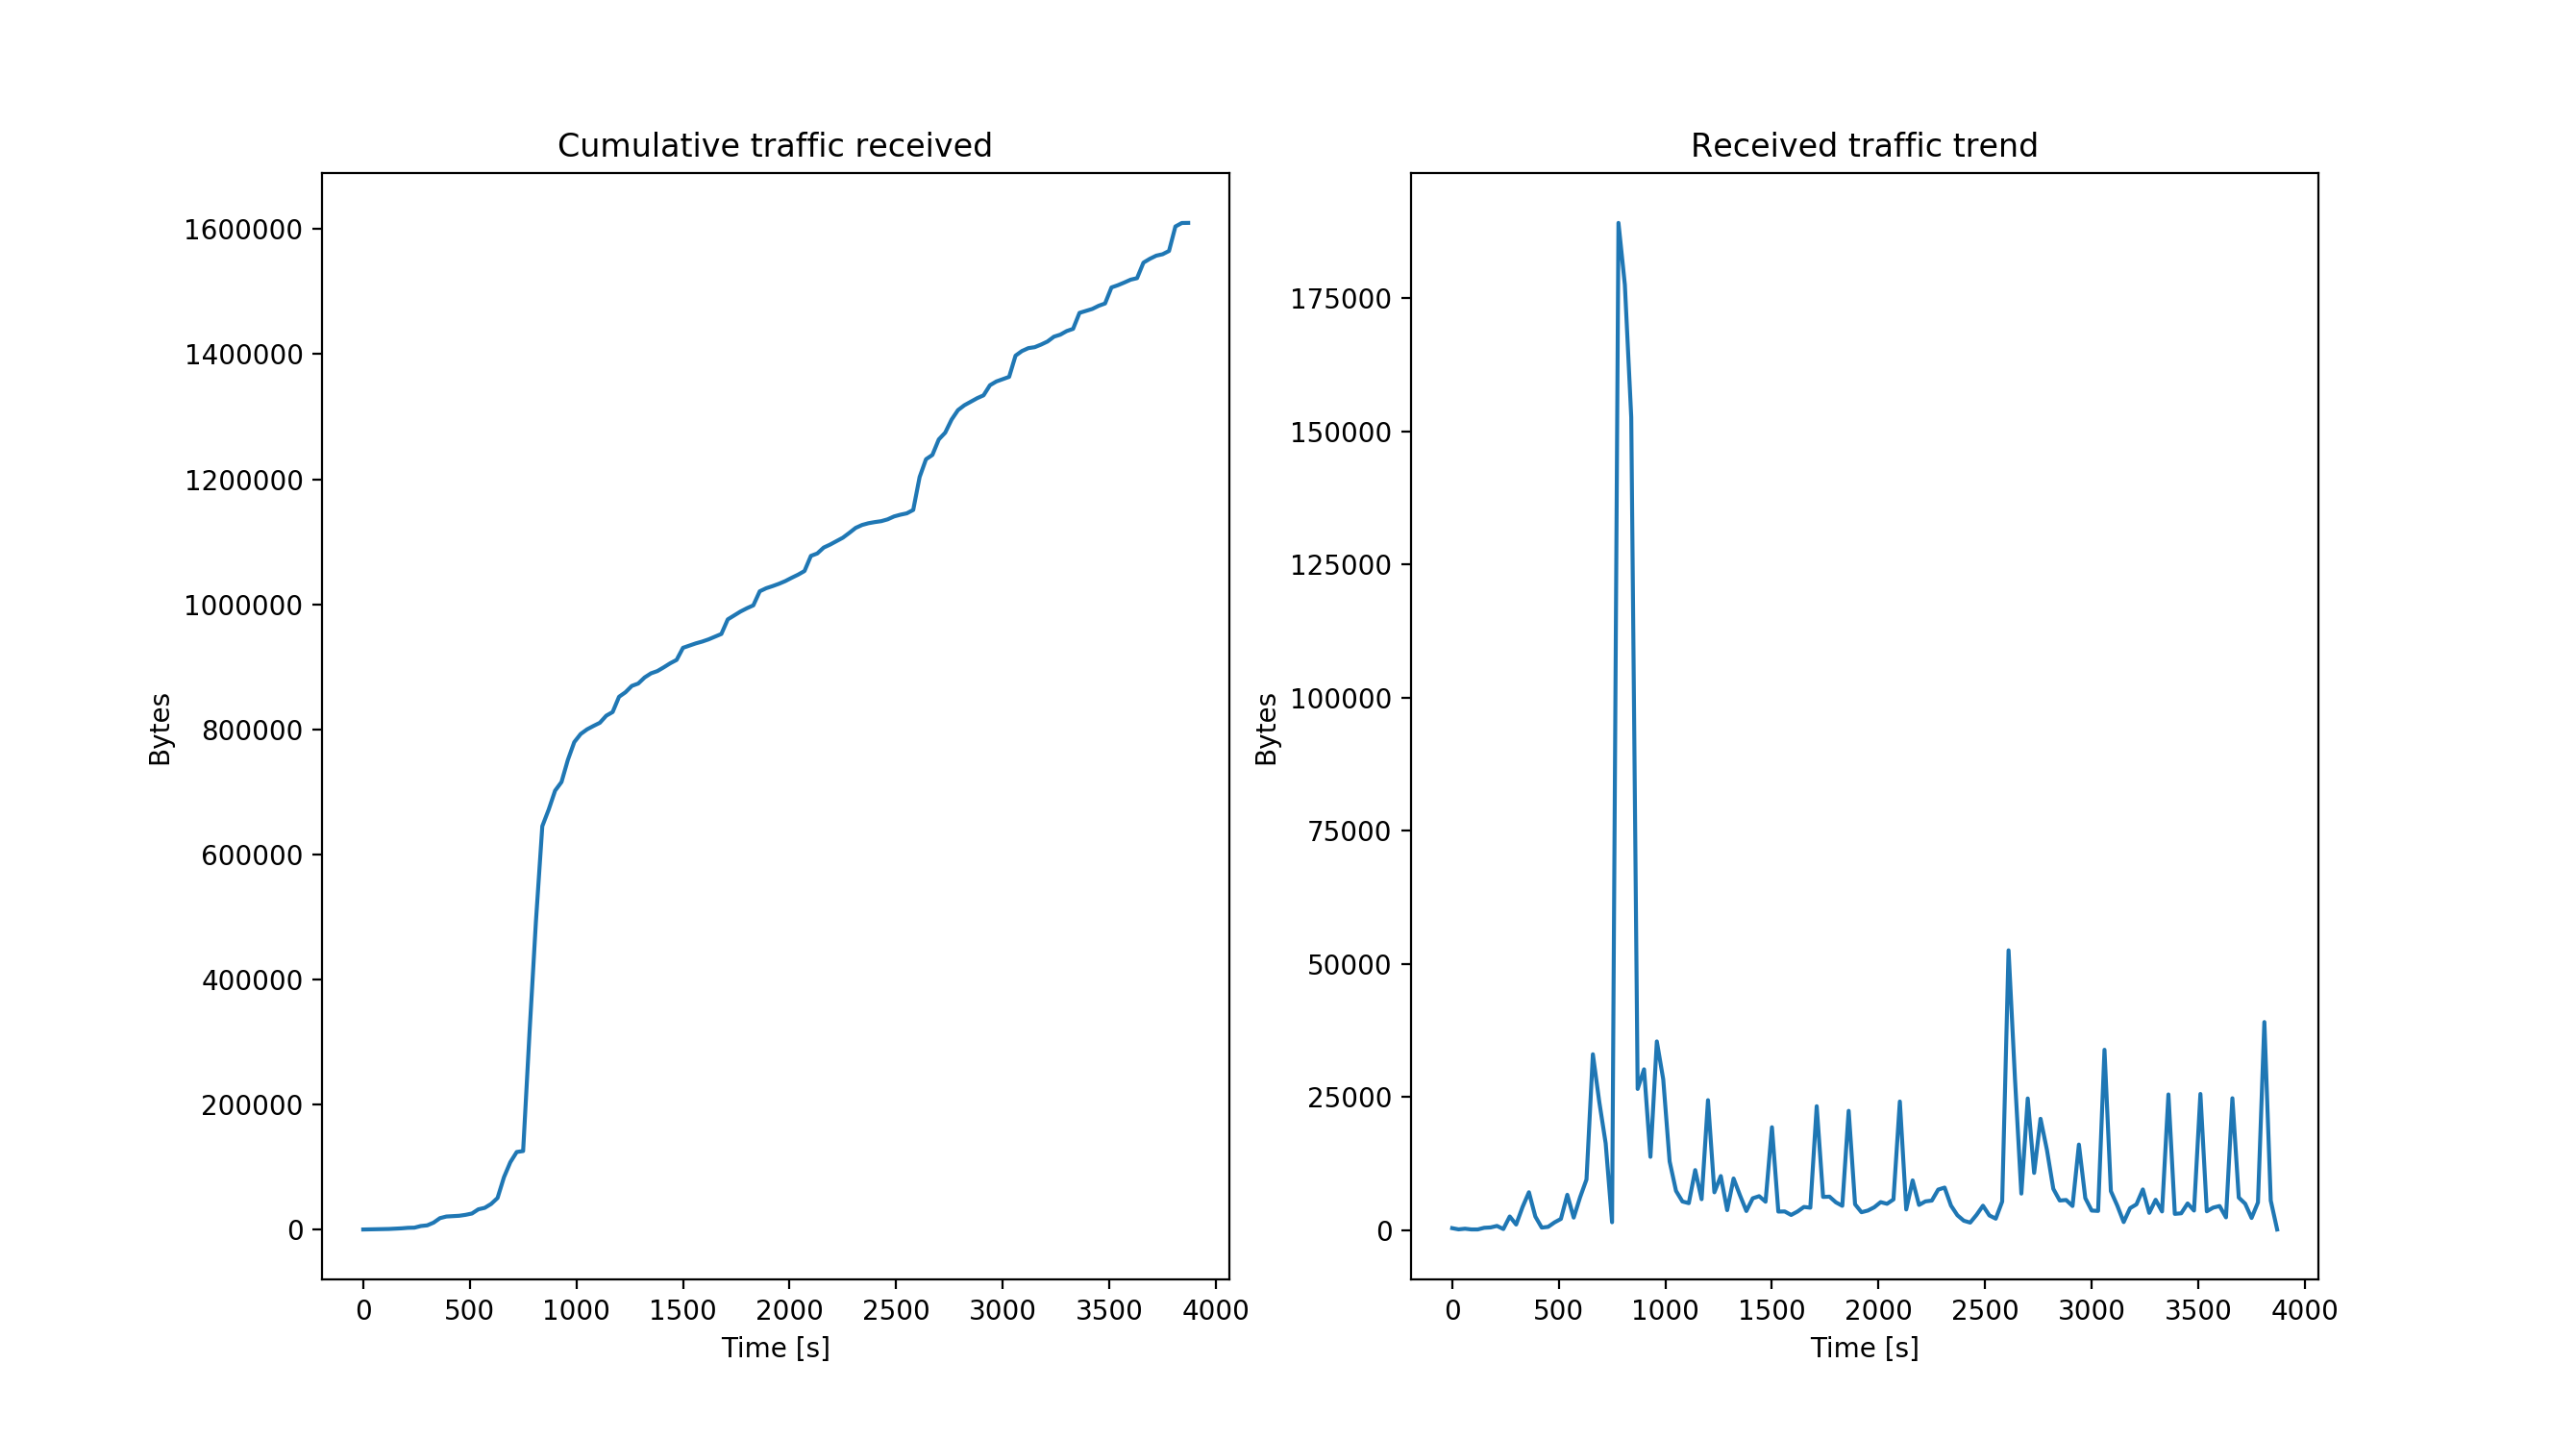
\includegraphics[width=\textwidth]{Graphs/SONOS_cum_in_traffic.png}
    \caption{Sonos input traffic graphs}
    \label{fig:Sonos_traffic}
\end{figure}
\\
To further show how many packets the Sonos devices exchanged we can see that three out of the four
devices are at the top spots of the following graph.
\begin{figure}[h]
    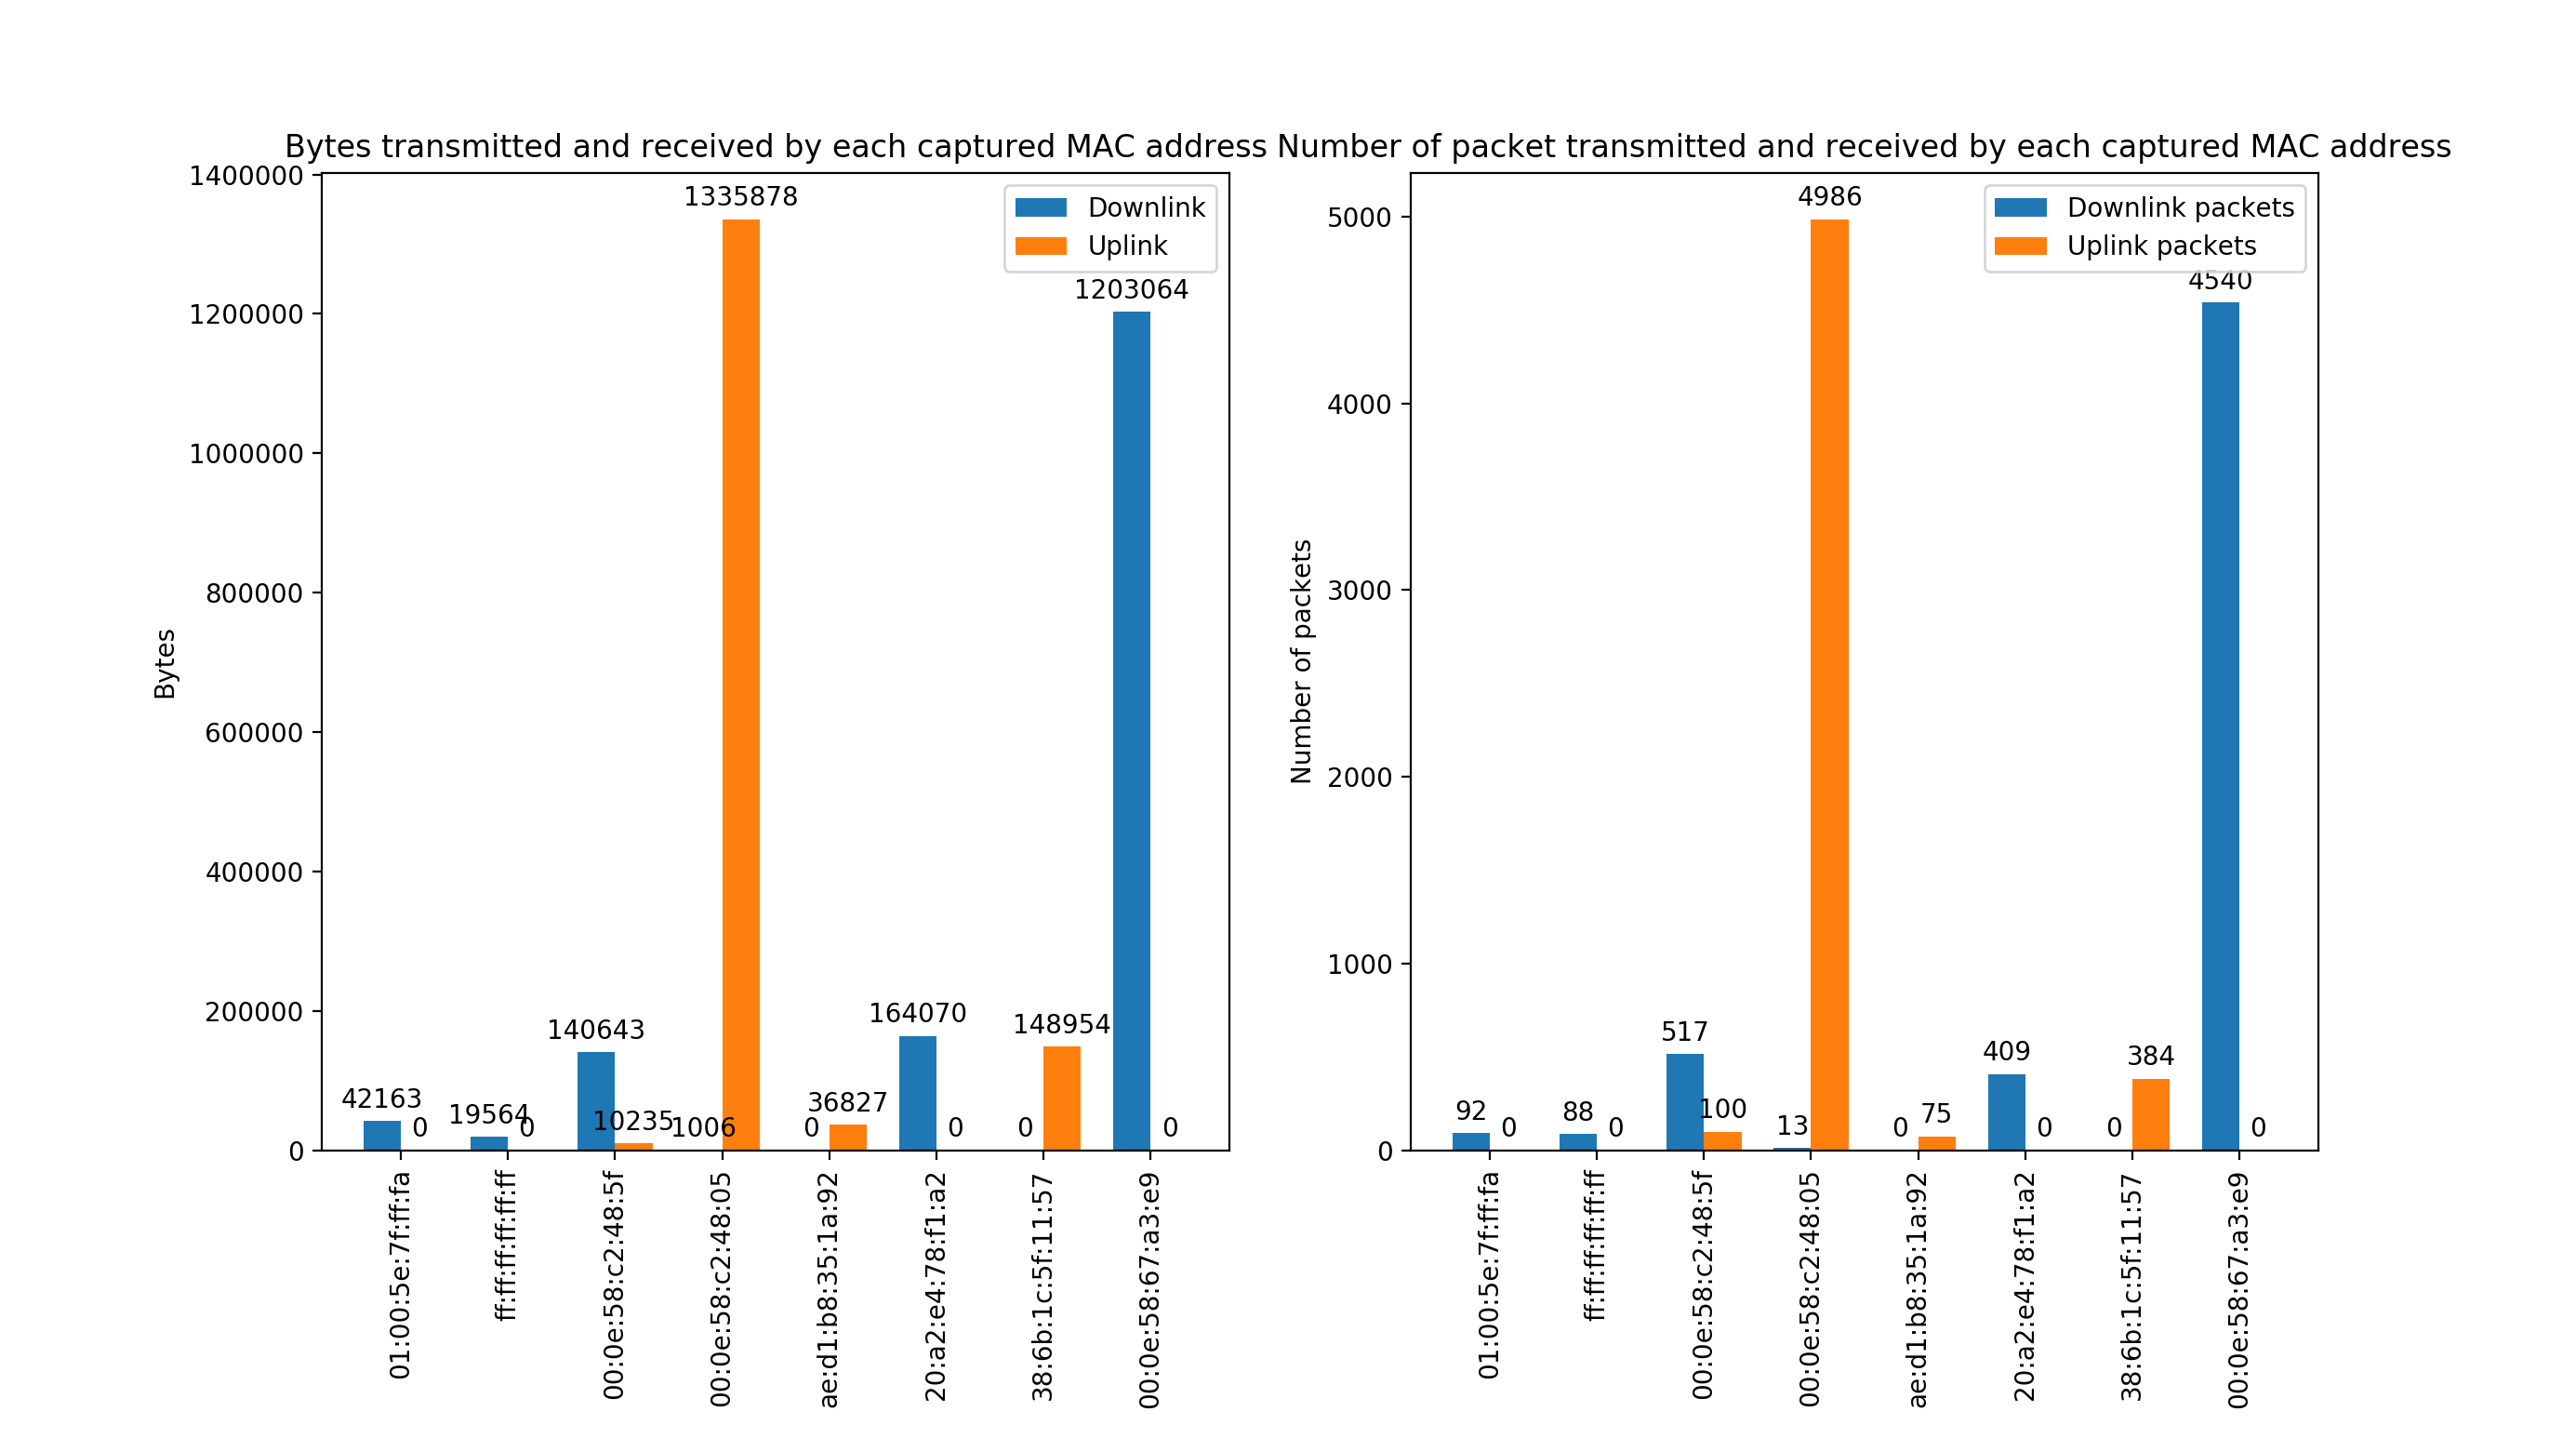
\includegraphics[width=\textwidth]{Graphs/SONOS_bytes_packets.png}
    \caption{Sonos packets exchanged}
    \label{fig:Sonos_packets}
\end{figure}


 
\subsection{ZOOM}
%Fabio

\subsection{MULTIMEDIA INTERNET}
%Luca

\subsection{LAUNCH TIME}
%Luca